\section{Beziehung von Stellgrößen der Motoren zu Lenkwinkel und Geschwindigkeit}
\subsection{Geschwindigkeit}
Um die Geschwindigkeit zu einer jeweils vorgegebenen Leistung am Motor zu bestimmen, haben wir das Auto auf gerader Strecke durch zwei Lichtschranken fahren lassen. Mithilfe eines Osziloskops konnten wir die Kurvenverläufe an den Ausgängen der Lichtschranken vergleichen und so die Zeit bestimmen, die das Auto gebraucht hat um die Strecke zwischen den beiden Schranken zurück zu legen. Mit einem aufgeklebten Papier an der Fahrzeugfront haben wir sichergestellt, dass trotz leichter Höhendifferenzen bei beiden Lichtschranken die erste Flanke des Ausgangssignals der gleichen Lage des Autos relativ zur Schranke entspricht.

Bezeichne $x(t): [0,\infty]\rightarrow \mathbb{R}$ die Lage des Autos in Fahrtrichtung, $l\in[0,\infty]$ den Abstand zwischen den beiden Lichtschranken und $t_1, t_2\in [0,\infty]$ den Zeitpunkt, bei dem die Fahrzeugfront an der ersten, beziehungsweise zweiten Lichtschranke ist. Dann lässt sich die Durschnittsgeschwindigkeit $v_d\in\mathbb{R}$ des Autos zwischen den beiden Schranken folgendermaßen berechnen:
\begin{equation*}
v_d := \frac{\int_{t_0}^{t_1}{\dot x(t) dt}}{t_1-t_0}=\frac{x(t_1)-x(t_2)}{t_1-t_0}=\frac{l}{t_1-t_0}
\end{equation*}
Wenn wir sicherstellen, dass das Auto zwischen den Schranken eine konstante Geschwindigkeit $v\in\mathbb{R}$ fährt, also $\dot x\vert_{t\in[t_0,t_1]}\equiv v$, entspricht $v_d=v$:
\begin{equation*}
v_d = \frac{\int_{t_0}^{t_1}{\dot x(t) dt}}{t_1-t_0} = \frac{\int_{t_0}^{t_1}{v dt}}{t_1-t_0}=v\frac{t_1-t_0}{t_1-t_0}=v
\end{equation*}
Falls die angenommenen Länge um $\Delta l\in\mathbb{R}$ von der wirklichen Länge $l$ abweicht ergibt sich ein Fehler $e\in \mathbb{R}$ bei der Bestimmung der Geschwindigkeit von
\begin{equation*}
	e = \frac{\Delta l}{t_1-t_0} = \frac{\Delta l}{\frac{l}{v}} = \frac{\Delta l}{l}v
\end{equation*}

Wir gehen davon aus, dass wir die Lichtschranken im Abstand von $1m\pm1cm$ genau plaziert haben, also deshalb die Geschwindigkeit bis auf $1\%$ genau bestimmen konnten. Den Messfehler bei der Zeitmessung betrachten wir hier nicht, da er sich mit dem Oszilloskop bis auf Mikrosekunden sehr genau bestimmen ließ. Die Messergebnisse sind im folgenden Graph dargestellt:

\begin{figure}[h]
\centering
% This file was created by matlab2tikz.
%
%The latest updates can be retrieved from
%  http://www.mathworks.com/matlabcentral/fileexchange/22022-matlab2tikz-matlab2tikz
%where you can also make suggestions and rate matlab2tikz.
%
\definecolor{mycolor1}{rgb}{0.00000,0.44700,0.74100}%
%
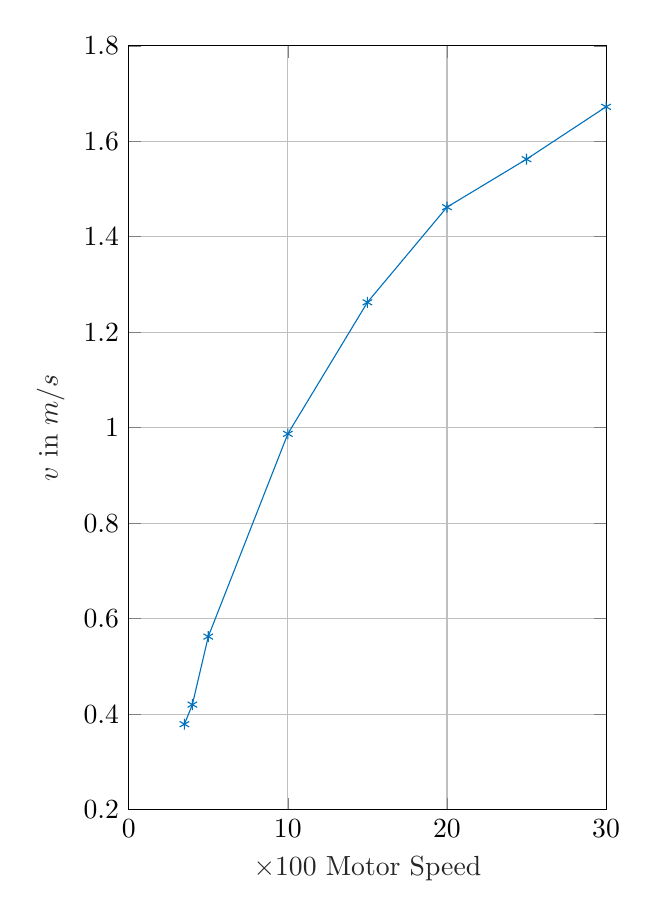
\begin{tikzpicture}

\begin{axis}[%
width=0.5\textwidth,
height=0.8\textwidth,
at={(0.758in,0.481in)},
scale only axis,
xmin=0,
xmax=30,
xlabel style={font=\color{white!15!black}},
xlabel={$\times 100$ Motor Speed},
ymin=0.2,
ymax=1.8,
ylabel style={font=\color{white!15!black}},
ylabel={$v$ in $m/s$},
axis background/.style={fill=white},
xmajorgrids,
ymajorgrids
]
\addplot [color=mycolor1, mark=asterisk, mark options={solid, mycolor1}, forget plot]
  table[row sep=crcr]{%
3.5	0.378931413414172\\
4	0.419991600167997\\
5	0.562429696287964\\
10	0.987166831194472\\
15	1.26262626262626\\
20	1.46198830409357\\
25	1.5625\\
30	1.67224080267559\\
};
\end{axis}
\end{tikzpicture}%
\caption[Motor Speed]{Geschwindigkeitsmessergebnisse für Simulink Stellgröße \texttt{Motor Speed}}
\label{fig:motor_speed}
\end{figure}

\subsection{Lenkwinkel}

Um den Lenkwinkel zu messen, haben wir die Reifenstellung auf ein Papier abgetragen und die jeweiligen Winkel mit dem Geodreieck gemessen. Aufgrund von Fehlern beim Abtragen sowie dem recht großen Spiel der Reifen bei fest gesetzten Lenkwinkel schätzen wir den Messfehler auf $\pm5^\circ$ ein. Aus den Messergebnissen kann man einen linearen Zusammenhang erahnen:

\begin{figure}[h]
\centering
% This file was created by matlab2tikz.
%
%The latest updates can be retrieved from
%  http://www.mathworks.com/matlabcentral/fileexchange/22022-matlab2tikz-matlab2tikz
%where you can also make suggestions and rate matlab2tikz.
%
\definecolor{mycolor1}{rgb}{0.00000,0.44700,0.74100}%
%
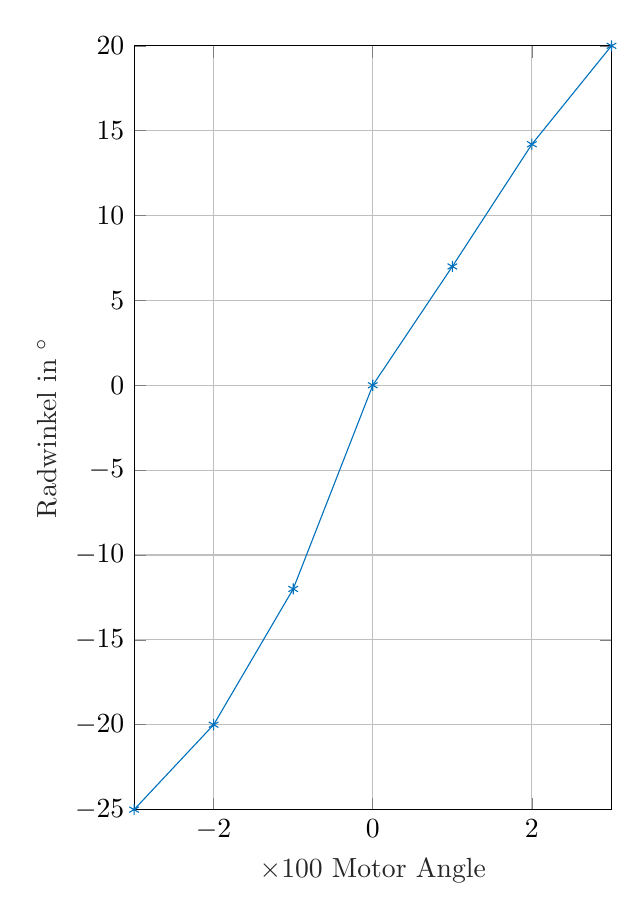
\begin{tikzpicture}

\begin{axis}[%
width=0.5\textwidth,
height=0.8\textwidth,
at={(0.758in,0.481in)},
scale only axis,
xmin=-3,
xmax=3,
xlabel style={font=\color{white!15!black}},
xlabel={$\times 100$ Motor Angle},
ymin=-25,
ymax=20,
ylabel style={font=\color{white!15!black}},
ylabel={Radwinkel in $^\circ$},
axis background/.style={fill=white},
xmajorgrids,
ymajorgrids
]
\addplot [color=mycolor1, mark=asterisk, mark options={solid, mycolor1}, forget plot]
  table[row sep=crcr]{%
-3	-25\\
-2	-20\\
-1	-12\\
0	0\\
1	7\\
2	14.2\\
3	20\\
};
\end{axis}
\end{tikzpicture}%
\caption[Motor Angle]{Lenkwinkelmessergebnisse für Simulink Stellgröße \texttt{Motor Angle}}
\label{fig:motor_angle}
\end{figure}

